\section{Clustering}
\label{sec:clustering}

In order to identify patterns in the trip data, we clustered trips using kmeans++ and gaussian mixture models. This can help in identifying local hot spots or recurring trips types such as commutes or leisure trips.

Kmeans++ is a hard clustering algorithm that assigns each data point to a definite cluster. Gaussian mixture models (GMMs), on the other  hand, are a soft clustering algorithm meaning we compute the probabilities of each data point belonging to each clusters. This gives us a measure of uncertainty. Moreover, while kmeans is mostly suited for capturing spherical shapes, GMM are also able to detect ellipsis shapes. However, non-convex shapes pose a difficulty for both algorithms. GMMs also tend to have longer computation times than kmeans due to the increased complexity.
In this section, we discuss the results of the hard clustering and soft clustering analysis. We clustered the data using all features in the first step and based on feature subsets in the second step. However, in this paper we only present the clustering using all features. We also omit plotting weather data, minimum distance and minimum average speed, which was also used in the clustering, as it did not yield any interesting insights.

\subsection{Hard Clustering - Kmeans++}
\label{sec:hard_clustering}

Based on the loss curve and for easier comparability we picked a total of five clusters. The plots depict the the differences between the cluster based on the latitude and longitude as well as temporal features (Figure \ref{fig:kmeans_loc_temp}), associated land use type (Figure \ref{fig:kmeans_land_use}), number of POIs (Figure \ref{fig:kmeans_poi}) for start and end location and some trip metrics (Table \ref{table:kmeans_trip_metrics}). 

\begin{longtable}{|l|c|c|c|c|c|}
    \hline
    \textbf{cluster} & \textbf{speed(mean)}  & \textbf{duration(mean/max)}   & \textbf{distance(mean)} \\
    \hline
    0 & 6.92 & 33.26/10497.0 & 1.86 \\
    \hline
    1 & 6.86 & 33.62/27376.0 & 1.80 \\
    \hline
    2 & 8.36 & 25.02/5272.0 & 2.00 \\
    \hline
    3 & 7.42 & 34.71/2693.0 & 1.95 \\
    \hline
    4 & 6.94 & 28.25/1376.0 & 1.66\\
    \hline

  \caption{Cluster Values for Speed(km/h), Duration(minutes) and Distance(km)}
  \label{table:kmeans_trip_metrics}
\end{longtable}


\begin{figure}[htp]
    \centering
    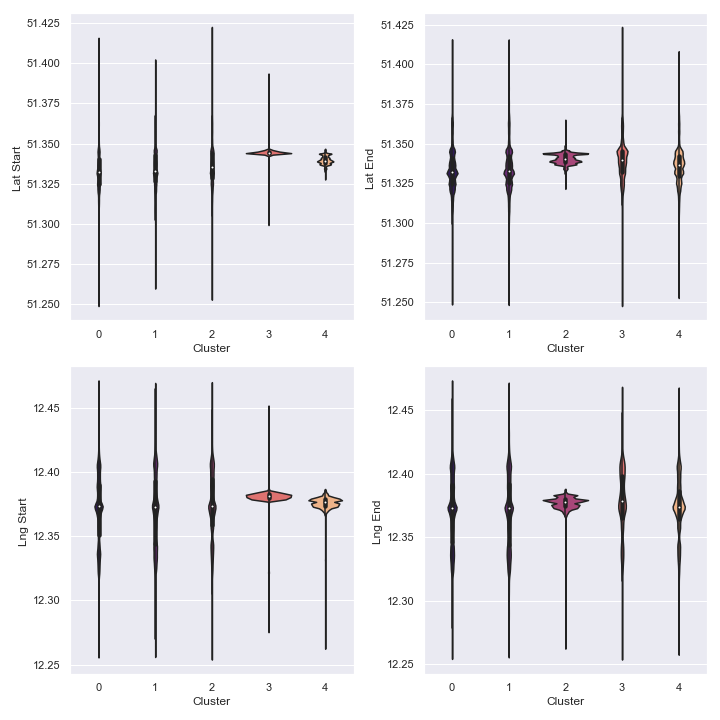
\includegraphics[width=0.48\textwidth]{Figures/Clustering/clusters_lat_start.png}
    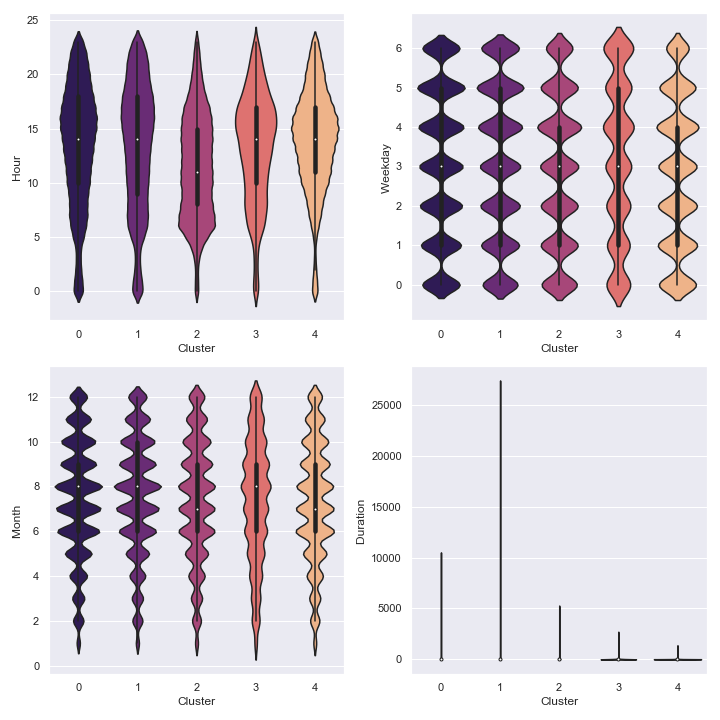
\includegraphics[width=0.48\textwidth]{Figures/Clustering/clusters_hour.png}
    \caption{Kmeans Clustering - Location And Temporal Features}
    \label{fig:kmeans_loc_temp}
\end{figure}
\begin{figure}[htp]
    \centering
    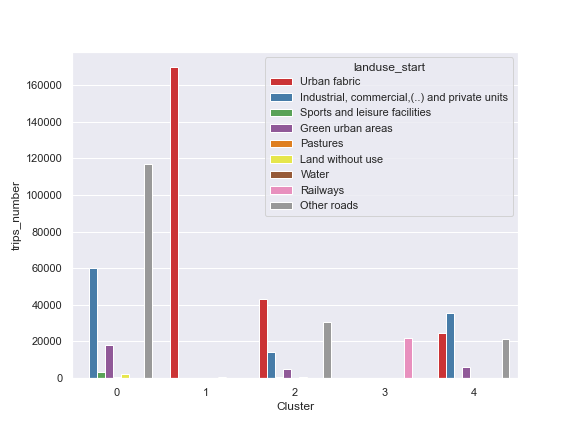
\includegraphics[width=0.48\textwidth]{Figures/Clustering/landuse_start.png}
    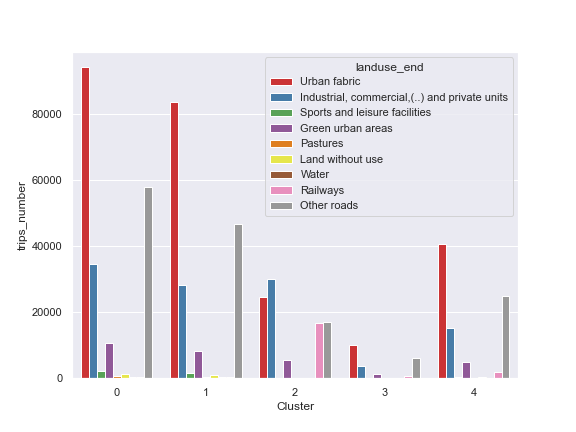
\includegraphics[width=0.48\textwidth]{Figures/Clustering/landuse_end.png}
    \caption{Kmeans Clustering - Land Use Start and End}
    \label{fig:kmeans_land_use}
\end{figure}
\begin{figure}[htp]
    \centering
    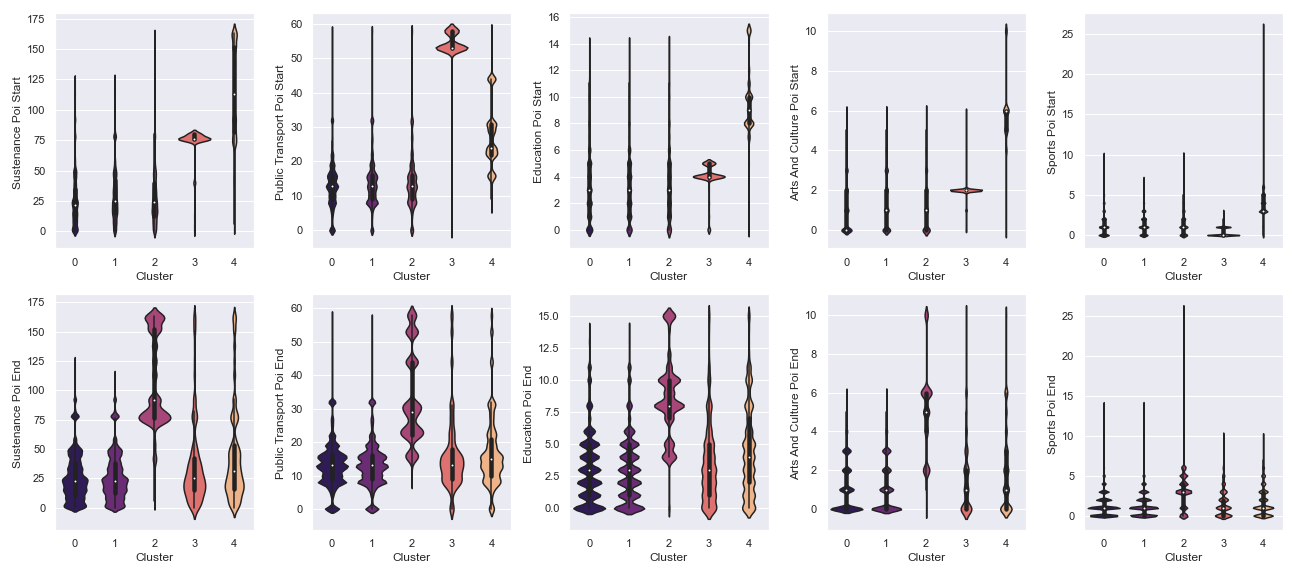
\includegraphics[width=1\textwidth]{Figures/Clustering/clusters_sustenance_poi_start.png}
    \caption{Kmeans Clustering - Points Of Interest}
    \label{fig:kmeans_poi}
\end{figure}


Cluster 0 is the largest cluster with a total of 202016 trips. They primarily start at roads (which is where bikes are usually parked) and end in urban fabric areas but vary across latitude and longitude. Cluster 1 does not contain the longest trips on average but does contain some long outlier trips. All trips from cluster 1 start in urban fabric areas. Both cluster 0 and cluster 1 contain more trips during the late evening and night than other cluster groups. They also tend to have a lower average speed. Cluster 2 is made up of trips that start in the city center. They also happen earlier in the day, are generally shorter in duration but higher in speed and occur less often on the weekend. It is also the only cluster group that often drives to railway areas, which could represent the train station. Moreover, a lot of trips end at different types of POIs such as sports, education or sustenance. This implies that these are people who either commute to different cities through the train station or to their work location within Leipzig (represented through a high number of POIs). Trips classified as cluster 3 go to the city center and start at the train station according to the land use type. This is supported by the fact that they also have a high average of public transport POIs at their start location. Because these trips happen more often in the afternoon and evening, it could be people commuting back home from work or visiting for leisure activities. The fact that they take place on all days of the week implies that this cluster is not solely work related. Cluster 4 also goes to the city center but starts and ends at various land use types. These trips also take place more often during the working week and in the afternoon. They start at various POIs such as arts/culture, sports or education. These characteristics also imply that these customers are using the bicycle to travel home from work or to and from their leisure activities in the city center. 

